% Netherlands CCyB group presentation (Frankfurt School, MSc FinTech)
% Build: cd slides && latexmk -pdf main.tex      (figures: python slides/figs.py from repo root)
% Storyline: docs/01_storyline.md (v4). Numbers: docs/02_findings.md.
\documentclass[aspectratio=169,11pt,t]{beamer}
\usetheme{default}
\usefonttheme{serif}
\geometry{papersize={20cm,11.25cm}}
\usepackage[T1]{fontenc}
\usepackage[utf8]{inputenc}
\usepackage{newpxtext,newpxmath}
\usepackage{textcomp,newunicodechar,booktabs,tabularx,array,colortbl,pifont,tikz,xcolor}
\usetikzlibrary{positioning,calc,arrows.meta,decorations.pathreplacing,shapes.symbols}

% ---------- unicode shortcuts
\newunicodechar{−}{\textminus}
\newunicodechar{→}{\ensuremath{\rightarrow}}
\newunicodechar{≈}{\ensuremath{\approx}}
\newunicodechar{×}{\ensuremath{\times}}
\newunicodechar{≤}{\ensuremath{\leq}}
\newunicodechar{½}{\ensuremath{\tfrac{1}{2}}}
\newunicodechar{€}{\texteuro}
\newunicodechar{✔}{\ensuremath{\checkmark}}
\newunicodechar{✘}{\ensuremath{\times}}

% ---------- palette: one accent (red = Netherlands), structure in dark blue, everything else grey
\definecolor{navy}{HTML}{1F3B73}
\definecolor{nlred}{HTML}{A93226}
\definecolor{gold}{HTML}{8C8C8C}      % kept as a name for diagrams; now a neutral grey
\definecolor{grey}{HTML}{6E6E6E}
\definecolor{light}{HTML}{E3E3E3}
\definecolor{okgreen}{HTML}{3A3A3A}   % kept as a name; now near-black
\setbeamercolor{normal text}{fg=black!88,bg=white}
\setbeamercolor{structure}{fg=navy}
\setbeamercolor{frametitle}{fg=navy,bg=}
\setbeamercolor{title}{fg=navy}
\setbeamercolor{alerted text}{fg=nlred}
\setbeamercolor{block title}{fg=navy,bg=}
\setbeamercolor{block body}{bg=}
\setbeamercolor{block title alerted}{fg=nlred,bg=}
\setbeamercolor{block body alerted}{bg=}
\setbeamercolor{block title example}{fg=black!80,bg=}
\setbeamercolor{block body example}{bg=}
\setbeamerfont{frametitle}{size=\large,series=\mdseries}
\setbeamerfont{block title}{size=\normalsize,series=\bfseries}
\setbeamersize{text margin left=0.7cm,text margin right=0.7cm}
\setbeamertemplate{navigation symbols}{}
\setbeamertemplate{blocks}[default]
\setbeamertemplate{itemize item}{\textendash}
\setbeamertemplate{itemize subitem}{\textendash}

% ---------- frame title: left-aligned, hairline rule, small grey section label (Q1/Q2/Q3)
\gdef\theqtag{}
\newcommand{\qtag}[1]{\gdef\theqtag{#1}}
\setbeamertemplate{frametitle}{%
  \vspace*{0.35cm}%
  \begin{minipage}[b]{0.82\textwidth}\raggedright\usebeamerfont{frametitle}\usebeamercolor[fg]{frametitle}\insertframetitle\end{minipage}%
  \hfill
  \begin{minipage}[b]{0.16\textwidth}\raggedleft\scriptsize\color{grey}\textsc{\theqtag}\end{minipage}\par
  \vspace{3pt}{\color{black!25}\rule{\textwidth}{0.3pt}}\vspace{4pt}}

% ---------- footline: authors left, page number right
\setbeamertemplate{footline}{%
  \hspace{0.7cm}{\color{grey}\fontsize{7}{8}\selectfont Huang \& Gutiérrez \,·\, The Netherlands' CCyB}%
  \hfill{\color{grey}\fontsize{7}{8}\selectfont\insertframenumber/\inserttotalframenumber}\hspace{0.7cm}\vspace{0.25cm}}

% ---------- title page
\setbeamertemplate{title page}{%
  \vspace*{1.2cm}
  {\color{navy}\fontsize{26}{30}\selectfont\inserttitle\par}
  \vspace{0.25cm}
  {\large\color{black!75}\insertsubtitle\par}
  \vspace{0.35cm}{\color{black!30}\rule{0.6\textwidth}{0.4pt}}\par\vspace{0.35cm}
  {\normalsize\insertauthor\par}\vspace{0.15cm}
  {\small\color{grey}\insertinstitute\par}\vspace{0.15cm}
  {\small\color{grey}\insertdate\par}}

% ---------- helpers
\newcommand{\source}[1]{%
  \begin{tikzpicture}[remember picture,overlay]
    \node[anchor=south west,inner sep=0pt,text width=0.86\paperwidth,align=left,font=\fontsize{6.5}{7.5}\selectfont,text=grey]
      at ($(current page.south west)+(0.7cm,0.62cm)$) {Source: #1};
  \end{tikzpicture}}
\newcommand{\kpi}[3]{% value, label, colour -- plain figure with caption, no box
  \begin{minipage}[t]{3.9cm}\centering
    {\LARGE\color{#3}#1}\\[3pt]{\scriptsize\color{black!70}#2}
  \end{minipage}}
\newcommand{\quot}[2]{{\itshape “#1”}\hfill{\scriptsize\color{grey}(#2)}}
\newcommand{\hl}[1]{\textcolor{nlred}{#1}}
\newcommand{\heading}[1]{{\color{navy}\textsc{#1}}\par\vspace{2pt}}
% takeaway: pushed to the bottom of the frame, short red rule, one or two full sentences
\newcommand{\takeaway}[1]{\par\vfill\noindent{\color{nlred}\rule{1.1cm}{0.7pt}}\par\vspace{3pt}{\color{black!85}#1}\par\vspace{0.72cm}}
\newcommand{\nv}[1]{\textcolor{navy}{\bfseries #1}}
\newcolumntype{L}[1]{>{\raggedright\arraybackslash}p{#1}}
\renewcommand{\arraystretch}{1.18}

\title{Refilling the Buffer in a Storm}
\subtitle{The Netherlands' countercyclical capital buffer, 0\% → 2\% (2022–2024)}
\author{Zheng Huang \quad·\quad Diego Gutiérrez}
\institute{Micro- \& Macroprudential Management · Country implementation of a CCyB increase\\[2pt]Master of Financial Technology · Frankfurt School of Finance \& Management}
\date{October 2026}

\begin{document}

% =====================================================================================
\begin{frame}[plain]
  \titlepage
\end{frame}

% ===================================================================================== 1
\qtag{Summary}
\begin{frame}{In 2022--23 the Netherlands raised its countercyclical capital buffer (CCyB) to 2\% while the rulebook said 0\%. It was refilling a buffer, not fighting a boom}
  \small
  De Nederlandsche Bank (DNB) raised the CCyB from 0\% to 1\% (announced May 2022) and then to \hl{2\%} (announced May 2023, binding since 31 May 2024). At both decisions the Basel reference indicator, the credit-to-GDP gap, stood far below zero (\nv{−33} and \nv{−47} percentage points), so the rulebook pointed to a buffer of 0\%.
  \vspace{8pt}
  \begin{columns}[T,onlytextwidth]
    \column{0.31\textwidth}
    \heading{Q1 · Environment}
    \footnotesize The economy had recovered from COVID, but war, an energy shock and 11.6\% inflation darkened the outlook, and the ECB began raising rates in July 2022. Credit was cold, housing was hot and then cooled, and the banks were strong and growing more profitable.
    \column{0.31\textwidth}
    \heading{Q2 · Criteria and risks}
    \footnotesize DNB's 2022 framework sets 2\% as the normal level, calibrated on past crisis losses rather than on credit growth. The buffer insures against shocks that no indicator predicts, while housing risks are handled by other tools. It also kept a promise made in March 2020.
    \column{0.31\textwidth}
    \heading{Q3 · Implications}
    \footnotesize The buffer was cheap, at most about a fifth of the big banks' spare capital. It was largely a swap for cuts in structural buffers, and we see no sign of a contraction in lending. The Netherlands now has €6.7bn it can release.
  \end{columns}
  \takeaway{Our verdict: \hl{normalisation, not tightening.} The price is a greater reliance on DNB's judgement, and the buffer has not yet been tested in a crisis.}
  \source{DNB (2020, 2022, 2023, 2026); DNB Financial Stability Reports 2022–23; BIS credit-to-GDP gaps; ECB; bank disclosures; own calculations.}
\end{frame}

% ===================================================================================== 2
\qtag{Prologue}
\begin{frame}{In March 2020 COVID struck and neighbours released their buffers, but the Dutch buffer was empty}
  \begin{columns}[T,onlytextwidth]
    \column{0.58\textwidth}
    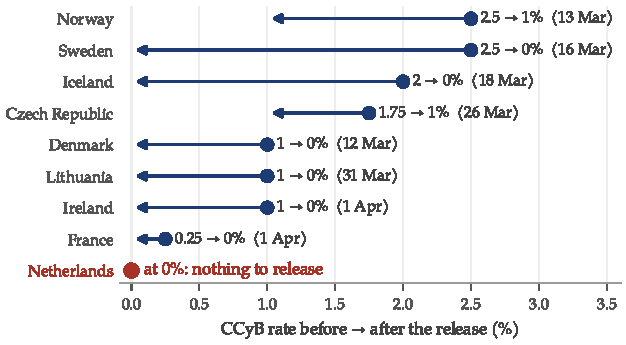
\includegraphics[width=\linewidth]{figs/releases.pdf}
    \column{0.38\textwidth}\small
    Within three weeks, eight European countries cut their countercyclical buffers so that banks could absorb losses and keep lending. Belgium and Germany cancelled increases they had already announced.\\[5pt]
    The Netherlands had nothing to release. DNB improvised: on 17 March 2020 it cut the systemic buffers of ING, Rabobank and ABN AMRO and postponed a planned floor on mortgage risk weights. This freed \nv{€8bn} of capital, enough to support up to \nv{€200bn} of lending.
  \end{columns}
  \takeaway{\textit{“Once the situation is back to normal, DNB will compensate the systemic buffers reduction by gradually increasing the countercyclical capital buffer to 2\%.”} \hfill{\footnotesize\color{grey}DNB, 17 March 2020}}
  \source{ESRB, CCyB rates table (announcements March–April 2020); DNB press release “DNB lowers bank buffer requirements to support lending”, 17 Mar 2020.}
\end{frame}

% ===================================================================================== 3
\qtag{Prologue}
\begin{frame}{That mattered because the CCyB is the only layer of bank capital an authority can release in a crisis}
  \begin{columns}[T,onlytextwidth]
    \column{0.46\textwidth}
    \centering\vspace{2pt}
    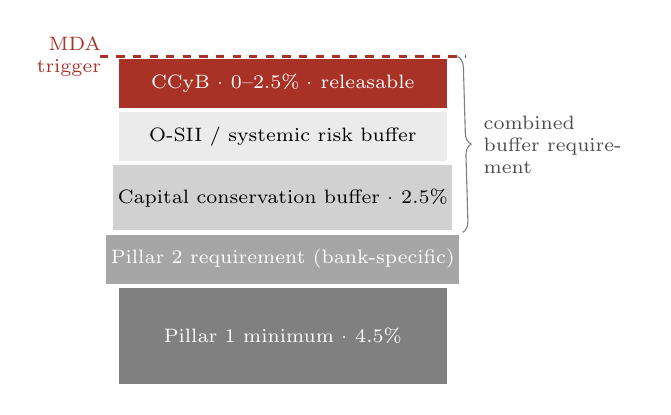
\begin{tikzpicture}[font=\scriptsize,box/.style={draw=white,thick,minimum width=4.2cm,align=center,inner sep=2pt}]
      \node[box,fill=black!50,text=white,minimum height=1.25cm] (p1) {Pillar 1 minimum · 4.5\%};
      \node[box,fill=black!35,text=white,minimum height=0.65cm,above=0pt of p1] (p2r) {Pillar 2 requirement (bank-specific)};
      \node[box,fill=black!18,minimum height=0.85cm,above=0pt of p2r] (ccob) {Capital conservation buffer · 2.5\%};
      \node[box,fill=black!8,minimum height=0.65cm,above=0pt of ccob] (osii) {O-SII / systemic risk buffer};
      \node[box,fill=nlred,text=white,minimum height=0.65cm,above=0pt of osii] (ccyb) {CCyB · 0–2.5\% · releasable};
      \draw[decorate,decoration={brace,amplitude=4pt},black!50] ([xshift=3pt]ccyb.north east) -- ([xshift=3pt]ccob.south east)
        node[midway,right=5pt,align=left,text width=1.9cm,text=black!70]{combined buffer requirement};
      \draw[nlred,thick,dashed] ([xshift=-6pt]ccyb.north west) -- ([xshift=6pt]ccyb.north east);
      \node[left=2pt of ccyb.north west,anchor=east,text=nlred,align=right] {MDA\\trigger};
    \end{tikzpicture}\\[2pt]
    {\tiny\color{grey}Capital stack in \% of risk-weighted assets (RWA), not to scale.}
    \column{0.50\textwidth}\small
    Read the stack from the bottom. Banks must always meet the minimum requirements; the buffers on top can be used in bad times.\\[5pt]
    If a bank's capital falls below the top of its buffers (the MDA trigger), its dividends and bonuses are restricted automatically. Banks therefore avoid using buffers even when they are allowed to. In COVID, banks close to this line cut lending instead.\\[5pt]
    The CCyB works differently. The authority can switch it off, so the requirement itself falls and the bank faces no penalty and no stigma. Increases bind only after twelve months, but a release is immediate.
  \end{columns}
  \takeaway{Only a buffer that the authority can \hl{release} is truly usable in a crisis, and it has to be filled beforehand.}
  \source{CRD (Arts.\ 130–136); BCBS (2024) d585; Couaillier, Lo Duca, Reghezza \& Rodriguez d'Acri (2022), ECB WP 2644.}
\end{frame}

% ===================================================================================== 4
\qtag{The question}
\begin{frame}{Two years later DNB refilled it in the middle of a storm and against its own rulebook. Was that the wrong moment?}
  \begin{columns}[T,onlytextwidth]
    \column{0.47\textwidth}\small
    \heading{The storm of 2022--23}
    Russia invaded Ukraine and energy prices hit records. Dutch inflation averaged 11.6\% in 2022, the ECB raised rates from July 2022, and house prices were about to fall. The Basel rule, based on the credit gap, said the buffer should be 0\%.
    \column{0.47\textwidth}\small
    \heading{The decision}
    DNB nevertheless raised the CCyB from 0\% to 1\% (announced May 2022) and then to 2\% (announced May 2023). Each step became binding a year later, in May 2023 and May 2024.
  \end{columns}
  \vspace{12pt}
  \begin{center}
    Raising capital requirements in a downturn can amplify the cycle, which is exactly\\ the \hl{procyclical mistake} the CCyB was invented to avoid. So was DNB tightening into a slowdown, fighting a hidden boom, or doing something else?
  \end{center}
  \vspace{6pt}
  \begin{center}
  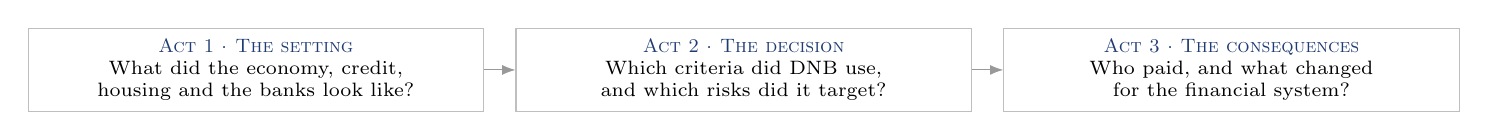
\begin{tikzpicture}[node distance=0.4cm,act/.style={draw=black!25,text width=5.5cm,minimum height=1.0cm,align=center,font=\scriptsize,inner sep=4pt}]
    \node[act] (a1) {{\color{navy}\textsc{Act 1 · The setting}}\\What did the economy, credit,\\housing and the banks look like?};
    \node[act,right=of a1] (a2) {{\color{navy}\textsc{Act 2 · The decision}}\\Which criteria did DNB use,\\and which risks did it target?};
    \node[act,right=of a2] (a3) {{\color{navy}\textsc{Act 3 · The consequences}}\\Who paid, and what changed\\for the financial system?};
    \draw[-{Latex},black!40] (a1)--(a2); \draw[-{Latex},black!40] (a2)--(a3);
  \end{tikzpicture}
  \end{center}
  \source{CBS (HICP 2022); ECB monetary policy decision, 21 Jul 2022; BIS credit-to-GDP gaps (latest data at each decision: 2021Q4, 2022Q4).}
\end{frame}

% ===================================================================================== 5
\qtag{Q1 · Environment}
\begin{frame}{The refill followed the path promised in 2020, one step per year, just as the ECB started to tighten}
  \centering\vspace{4pt}
  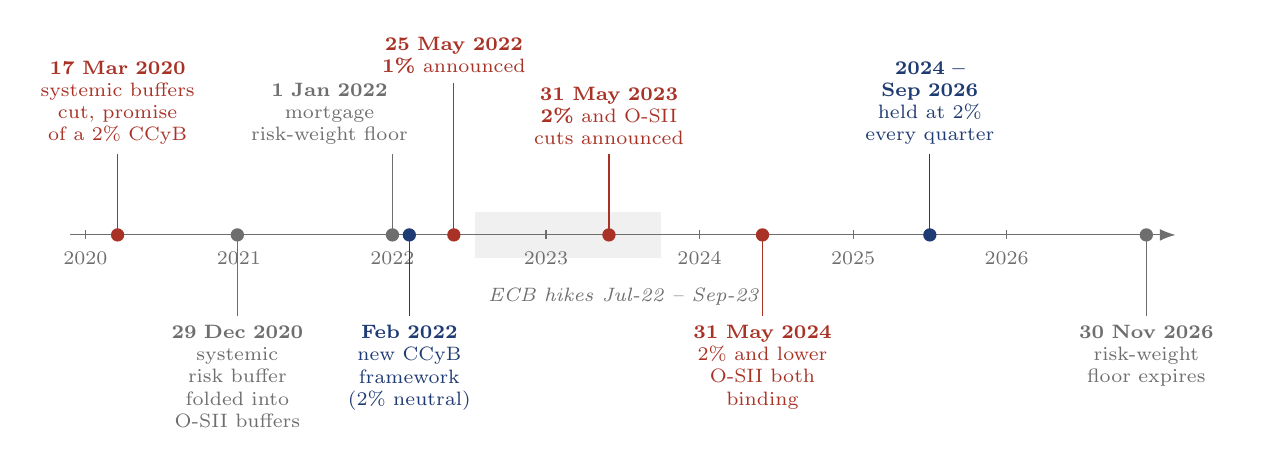
\begin{tikzpicture}[x=1.95cm,y=0.82cm,font=\scriptsize]
    \fill[black!6] (2.54,-0.35) rectangle (3.75,0.35);
    \node[text=grey,font=\scriptsize\itshape,anchor=west] at (2.56,-0.95) {ECB hikes Jul-22 – Sep-23};
    \draw[-{Latex[length=2mm]},grey] (-0.1,0)--(7.1,0);
    \foreach \y/\x in {2020/0,2021/1,2022/2,2023/3,2024/4,2025/5,2026/6}{\draw[grey](\x,0.07)--(\x,-0.07) node[below=1pt]{\y};}
    \fill[nlred] (0.21,0) circle (2.4pt); \draw[nlred] (0.21,0)--(0.21,1.25) node[above,align=center,text width=2.05cm]{\textbf{17 Mar 2020}\\systemic buffers cut, promise of a 2\% CCyB};
    \fill[grey] (0.99,0) circle (2.4pt); \draw[grey] (0.99,0)--(0.99,-1.25) node[below,align=center,text width=2.05cm]{\textbf{29 Dec 2020}\\systemic risk buffer folded into O-SII buffers};
    \fill[grey] (2.0,0) circle (2.4pt); \draw[grey] (2.0,0)--(2.0,1.25) node[above left=0pt and -0.35cm,align=center,text width=2.05cm]{\textbf{1 Jan 2022}\\mortgage risk-weight floor};
    \fill[navy] (2.11,0) circle (2.4pt); \draw[navy] (2.11,0)--(2.11,-1.25) node[below,align=center,text width=2.05cm]{\textbf{Feb 2022}\\new CCyB framework (2\% neutral)};
    \fill[nlred] (2.40,0) circle (2.4pt); \draw[nlred] (2.40,0)--(2.40,2.35) node[above,align=center,text width=2.05cm]{\textbf{25 May 2022}\\\textbf{1\%} announced};
    \fill[nlred] (3.41,0) circle (2.4pt); \draw[nlred] (3.41,0)--(3.41,1.25) node[above,align=center,text width=2.05cm]{\textbf{31 May 2023}\\\textbf{2\%} and O-SII cuts announced};
    \fill[nlred] (4.41,0) circle (2.4pt); \draw[nlred] (4.41,0)--(4.41,-1.25) node[below,align=center,text width=2.05cm]{\textbf{31 May 2024}\\2\% and lower O-SII both binding};
    \fill[navy] (5.5,0) circle (2.4pt); \draw[navy] (5.5,0)--(5.5,1.25) node[above,align=center,text width=2.05cm]{\textbf{2024 – Sep 2026}\\held at 2\% every quarter};
    \fill[grey] (6.91,0) circle (2.4pt); \draw[grey] (6.91,0)--(6.91,-1.25) node[below,align=center,text width=2.05cm]{\textbf{30 Nov 2026}\\risk-weight floor expires};
  \end{tikzpicture}
  \raggedright
  \takeaway{DNB moved in two equal steps of one percentage point, a year apart, and then stopped at 2\%. The first step was announced two months before the ECB's first rate hike.}
  \source{DNB press releases (17 Mar 2020; 27 May 2022; 31 May 2023; 24 Apr 2026; 17 Sep 2026); ESRB O-SII notifications (27 Nov 2020; 31 May 2023); ECB (21 Jul 2022; 14 Sep 2023).}
\end{frame}

% ===================================================================================== 6
\qtag{Q1 · Environment}
\begin{frame}{By then the economy had fully recovered, but war, energy prices and inflation were darkening the outlook}
  \centering
  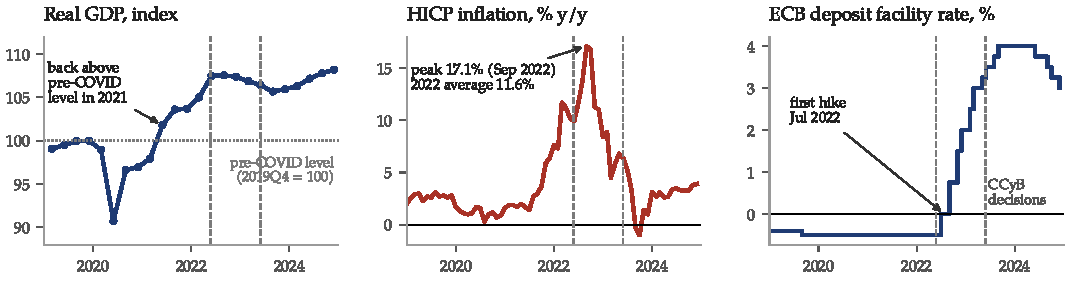
\includegraphics[width=\textwidth]{figs/macro.pdf}\par
  \raggedright\small\vspace{4pt}
  GDP was back above its pre-COVID level in 2021, which is the condition DNB's framework sets before a buffer is built. Then inflation rose to a peak of 17.1\%, and the ECB moved its deposit rate from −0.5\% to 4\% in fourteen months. DNB wrote in spring 2022 that \emph{“the economic outlook has worsened due to the war in Ukraine and high inflation.”}
  \takeaway{The macro picture argued both ways: build the buffer while the economy can take it, or wait because it is weakening.}
  \source{ECB Data Portal (Dutch real GDP, MNA; Dutch HICP, ICP; deposit facility rate, FM), current vintage; DNB Financial Stability Report, spring 2022. Dashed lines: CCyB announcements.}
\end{frame}

% ===================================================================================== 7
\qtag{Q1 · Environment}
\begin{frame}{In the financial system credit was cold and only housing was hot, and even housing soon turned}
  \centering
  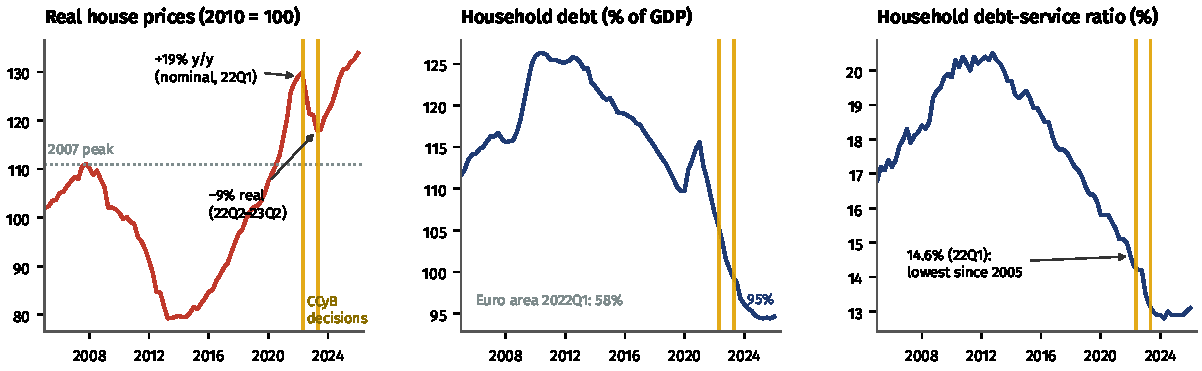
\includegraphics[width=\textwidth]{figs/indicators.pdf}\par
  \raggedright\small\vspace{2pt}
  \begin{columns}[T,onlytextwidth]
    \column{0.48\textwidth}
    Housing was hot. Nominal prices rose 19\% in the year to early 2022, and DNB itself wrote that \emph{“the overheated housing market calls for further measures.”} As mortgage rates rose, real prices fell by 9\%.
    \column{0.48\textwidth}
    Credit was not. Household debt is high (107\% of GDP against 58\% in the euro area) but it was falling, and the share of income spent on debt service was the lowest since 2005.
  \end{columns}
  \takeaway{If there was a boom, it was in house prices, not in credit.}
  \source{BIS (WS\_SPP, WS\_TC, WS\_DSR); DNB Financial Stability Report, spring 2022; own calculations. Dashed lines: CCyB announcements (May 2022, May 2023).}
\end{frame}

% ===================================================================================== 8
\qtag{Q1 · Environment}
\begin{frame}{Banks entered this storm well capitalised, and rising rates were lifting their profits}
  \centering
  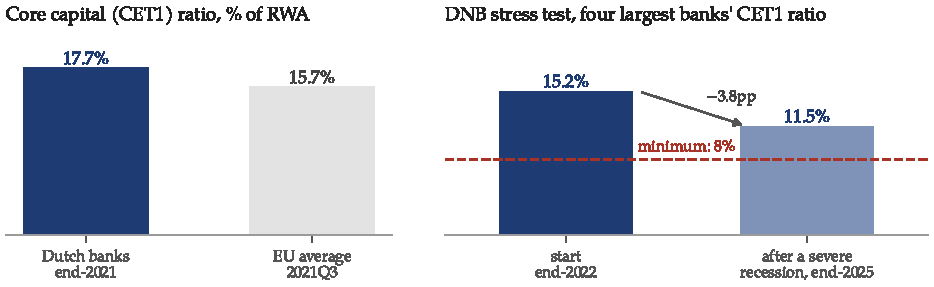
\includegraphics{figs/banks.pdf}\par
  \raggedright\small\vspace{4pt}
  Dutch banks held more core capital than the EU average, and in DNB's stress test the four largest banks stayed well above the minimum after a severe recession. Rising rates also lifted their net interest income, by 6.7\% in 2022; DNB had expected higher rates to \emph{“ultimately have a positive impact on the profitability of financial institutions.”}
  \takeaway{Act 1 in one sentence: war, inflation, rate hikes and a turning housing market argued against raising the buffer, while a recovered economy, cold credit and strong banks argued for it.}
  \source{DNB Financial Stability Reports, spring 2022 (CET1 17.7\%, EU 15.7\%) and spring 2023 (stress test, net interest income).}
\end{frame}

% ===================================================================================== 9
\qtag{Q2 · Criteria \& risks}
\begin{frame}{So why ignore the rulebook? On Dutch data the Basel rule had missed the last crisis and raised false alarms}
  \centering
  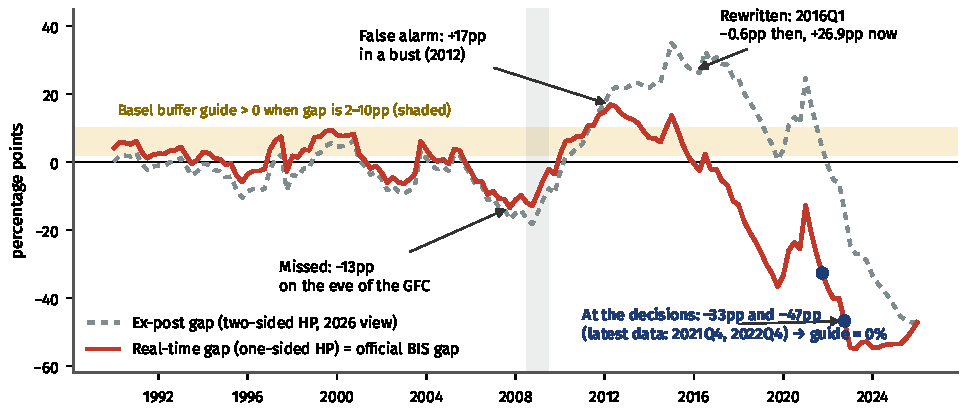
\includegraphics[width=\textwidth]{figs/gap.pdf}\par
  \raggedright\small\vspace{2pt}
  The credit-to-GDP gap measures how far credit relative to GDP is above its long-run trend. Under the Basel guide the buffer starts when the gap exceeds 2 points and reaches 2.5\% at 10 points.
  \takeaway{On Dutch data the gap missed the 2008 crisis, sounded a false alarm in 2012 and was later revised. At the two decisions it read −33 and −47 points.}
  \source{BIS credit-to-GDP gaps (Q.NL.P.A); Drehmann et al.\ (2010); Edge \& Meisenzahl (2011); own one-sided HP filter ($\lambda=400{,}000$).}
\end{frame}

% ===================================================================================== 10
\qtag{Q2 · Criteria \& risks}
\begin{frame}{DNB used its own compass instead: 2\% in normal times, calibrated on past crisis losses rather than on credit growth}
  \centering\vspace{6pt}
  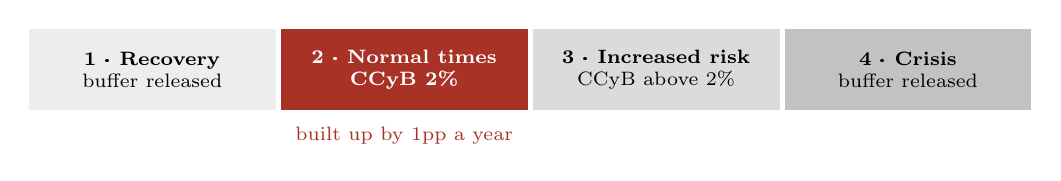
\begin{tikzpicture}[font=\scriptsize,ph/.style={draw=white,minimum height=1.05cm,minimum width=3.15cm,align=center,inner sep=2pt}]
    \node[ph,fill=black!7] (a) {\textbf{1 · Recovery}\\buffer released};
    \node[ph,fill=nlred,text=white,right=1pt of a] (b) {\textbf{2 · Normal times}\\\textbf{CCyB 2\%}};
    \node[ph,fill=black!14,right=1pt of b] (c) {\textbf{3 · Increased risk}\\CCyB above 2\%};
    \node[ph,fill=black!24,right=1pt of c] (d) {\textbf{4 · Crisis}\\buffer released};
    \node[below=2pt of b,text=nlred] {built up by 1pp a year};
  \end{tikzpicture}
  \vspace{12pt}

  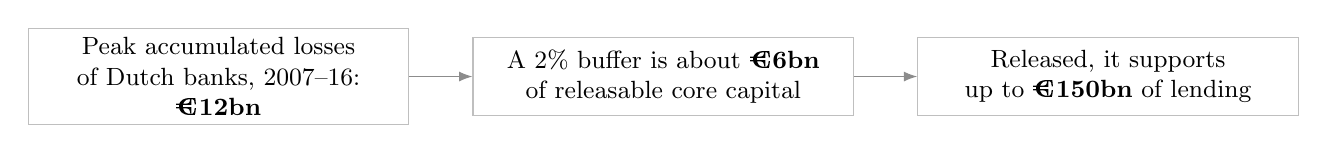
\begin{tikzpicture}[st/.style={draw=black!25,minimum height=1.0cm,text width=4.6cm,align=center,font=\small}]
    \node[st] (x) {Peak accumulated losses\\of Dutch banks, 2007–16:\\\textbf{€12bn}};
    \node[st,right=0.8cm of x] (y) {A 2\% buffer is about \textbf{€6bn}\\of releasable core capital};
    \node[st,right=0.8cm of y] (z) {Released, it supports\\up to \textbf{€150bn} of lending};
    \draw[-{Latex},black!45](x)--(y); \draw[-{Latex},black!45](y)--(z);
  \end{tikzpicture}
  \raggedright\small\vspace{10pt}

  The framework sets the buffer at 2\% when risks are neither high nor low, a so-called \emph{positive neutral} buffer. DNB reads a dashboard of indicators but stresses that there is \emph{“no mechanical link … guided discretion.”} Seventeen jurisdictions now work this way, and Sweden, the UK and Poland also target 2\%.
  \takeaway{The 2\% is sized to absorb about half of past crisis losses. It does not depend on credit growth.}
  \source{DNB (2022), Analytical framework for setting the CCyB in the Netherlands; BCBS (2024) d585, Table 1.}
\end{frame}

% ===================================================================================== 11
\qtag{Q2 · Criteria \& risks}
\begin{frame}{Its stated reasons were recovery, uncertainty and the 2020 promise, never credit growth}
  \begin{columns}[T,onlytextwidth]
    \column{0.47\textwidth}\small
    \heading{May 2022 · from 0\% to 1\%}
    {\itshape “When the systemic risk buffers \ldots{} were lowered in March 2020, we also announced our intention to \textbf{restore the buffers} by raising the CCyB.”}\\[5pt]
    {\itshape “The risk profile is currently dominated by uncertainty caused by the war in Ukraine, but \ldots{} the robust economic recovery \ldots{} provides grounds for a gradual build-up.”}\\[5pt]
    DNB judged cyclical risks to be normal to elevated.
    \column{0.47\textwidth}\small
    \heading{May 2023 · from 1\% to 2\%}
    {\itshape “Although the credit-to-GDP gap shows \textbf{no signs of excessive credit growth}, some other indicators already point to higher cyclical risk.”}\\[5pt]
    DNB cited investors' rising appetite for risk, falling real-estate prices, the debt sustainability of firms and governments, and banks that were \emph{“robust, partly due to rising interest rates.”}
  \end{columns}
  \takeaway{Both decisions rested on the same three pillars: a normal-to-elevated risk picture, strong banks and the 2020 promise. Credit growth was never the reason.}
  \source{DNB Financial Stability Report, spring 2022; DNB press releases of 27 May 2022 and 31 May 2023.}
\end{frame}

% ===================================================================================== 12
\qtag{Q2 · Criteria \& risks}
\begin{frame}{The buffer was meant for shocks nobody can forecast, while the known hot spots got their own tools}
  \centering\vspace{4pt}
  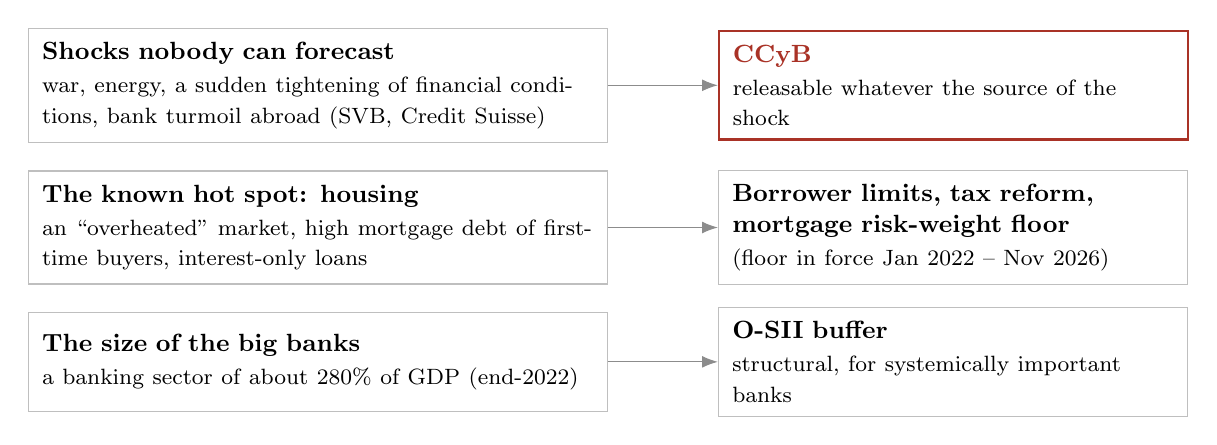
\begin{tikzpicture}[font=\small,
      risk/.style={draw=black!25,text width=7.0cm,minimum height=1.25cm,align=left,inner sep=5pt},
      tool/.style={text width=5.6cm,minimum height=1.25cm,align=left,inner sep=5pt},
      arr/.style={-{Latex[length=2mm]},black!45}]
    \node[risk] (r1) {\textbf{Shocks nobody can forecast}\\[1pt]\footnotesize war, energy, a sudden tightening of financial conditions, bank turmoil abroad (SVB, Credit Suisse)};
    \node[risk,below=0.35cm of r1] (r2) {\textbf{The known hot spot: housing}\\[1pt]\footnotesize an “overheated” market, high mortgage debt of first-time buyers, interest-only loans};
    \node[risk,below=0.35cm of r2] (r3) {\textbf{The size of the big banks}\\[1pt]\footnotesize a banking sector of about 280\% of GDP (end-2022)};
    \node[tool,draw=nlred,thick,right=1.4cm of r1] (t1) {\textbf{\color{nlred}CCyB}\\[1pt]\footnotesize releasable whatever the source of the shock};
    \node[tool,draw=black!25,right=1.4cm of r2] (t2) {\textbf{Borrower limits, tax reform, mortgage risk-weight floor}\\[1pt]\footnotesize (floor in force Jan 2022 – Nov 2026)};
    \node[tool,draw=black!25,right=1.4cm of r3] (t3) {\textbf{O-SII buffer}\\[1pt]\footnotesize structural, for systemically important banks};
    \draw[arr] (r1)--(t1); \draw[arr] (r2)--(t2); \draw[arr] (r3)--(t3);
  \end{tikzpicture}
  \raggedright
  \takeaway{One instrument per target, as the Tinbergen principle suggests. If housing had been the target, the CCyB would be the wrong tool, because it raises the cost of all lending, not only mortgages.}
  \source{DNB Financial Stability Reports, spring 2022 and spring 2023; ESRB O-SII notification NL (31 May 2023); DNB (24 Apr 2026); Tinbergen (1952).}
\end{frame}

% ===================================================================================== 13
\qtag{Q2 · Criteria \& risks}
\begin{frame}{Tested against the evidence, every prediction fits normalisation and none fits overheating}
  \centering\small
  \renewcommand{\arraystretch}{1.25}\begin{tabular}{@{}L{3.9cm}L{3.5cm}L{3.5cm}L{4.6cm}c@{}}
    \toprule
    & \textbf{If DNB was normalising} & \textbf{If DNB was fighting a boom} & \textbf{What actually happened} & \\
    \midrule
    Credit indicators & the buffer ignores them & the buffer rises with them & the indicators fell while the buffer rose & ✔ \\
    The path & +1pp a year, stop at 2\% & follows the risk & 1\%, then 2\%, then held & ✔ \\
    2023: prices falling, rates jumping & raise anyway & pause & DNB raised & ✔ \\
    2024–26: house prices up 10\% again & stay at 2\% & go above 2\% & held at 2\% & ✔ \\
    Other buffers & cut structural buffers in return & keep them & cut in 2020 and 2024 & ✔ \\
    \bottomrule
  \end{tabular}
  \raggedright
  \takeaway{Five predictions, five matches for \hl{normalisation}. The last row is the key to the next slide.}
  \source{BIS (WS\_CREDIT\_GAP, WS\_DSR, WS\_TC, WS\_SPP); DNB press releases 2022–2026 (house prices: DNB, 26 Mar 2026); DNB framework (2022); ESRB O-SII notifications.}
\end{frame}

% ===================================================================================== 14
\qtag{Q2 · Criteria \& risks}
\begin{frame}{And the refill was a swap, not a squeeze: capital moved from structural buffers into the releasable one}
  \begin{columns}[T,onlytextwidth]
    \column{0.56\textwidth}
    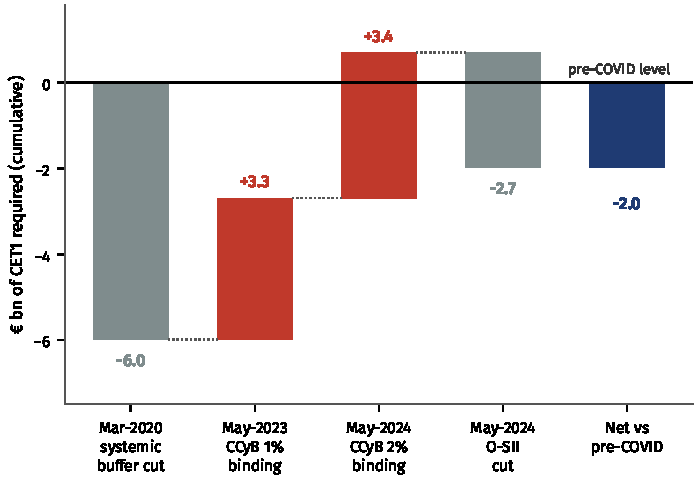
\includegraphics[width=\linewidth]{figs/swap.pdf}
    \column{0.40\textwidth}\small
    By our estimate, the 2020 cut released about €6bn and the 2024 cut another €2.7bn, while the two CCyB steps added €3.3bn and €3.4bn. Measured against the pre-COVID requirement, banks hold roughly the same amount of capital, or slightly less.\\[5pt]
    DNB described the swap as \emph{“more or less capital-neutral for the three large banks”} (2020) and later as \emph{“a limited increase in the net capital requirements”} (Knot, 2023).
  \end{columns}
  \takeaway{Capital moved from buffers that cannot be released into one that can. Relative to 2021, however, it was a modest increase.}
  \source{Own calculation (cuts valued at end-2022 RWA of the four largest banks; CCyB amounts: DNB, sector-wide); DNB (17 Mar 2020); Knot (7 Jun 2023).}
\end{frame}

% ===================================================================================== 15
\qtag{Q3 · Implications}
\begin{frame}{So was it the wrong moment? No. Higher rates gave banks the profits to build the buffer cheaply}
  \centering
  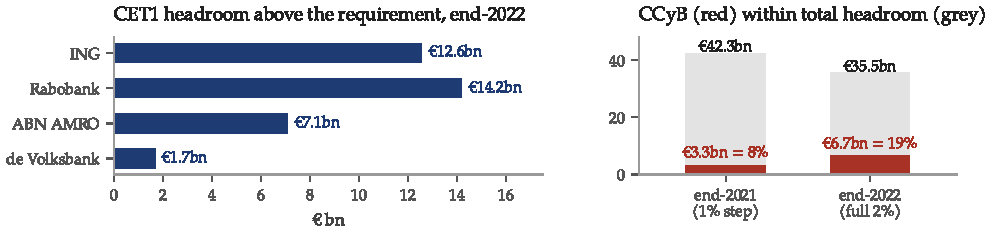
\includegraphics{figs/headroom.pdf}\par
  \raggedright\small\vspace{2pt}
  Headroom is the core capital a bank holds above its requirement. The four largest banks had €35.5bn of it at the end of 2022, so the full buffer of €6.7bn used at most a fifth. Higher net interest income meant the buffer could be built from retained earnings rather than by cutting loans, and the ECB finds that a gradual build-up by profitable banks keeps the costs low.
  \takeaway{It was not the wrong moment. Arguably it was the right one.}
  \source{Bank disclosures (ING, Rabobank, ABN AMRO, de Volksbank, 2021–22), de Volksbank requirement derived; DNB FSR 2023; ECB Macroprudential Bulletin 24 (2024) and 31 (2025, Box 2).}
\end{frame}

% ===================================================================================== 16
\qtag{Q3 · Implications}
\begin{frame}{Borrowers did not pay either: credit kept flowing and its price moved with the rest of the euro area}
  \centering
  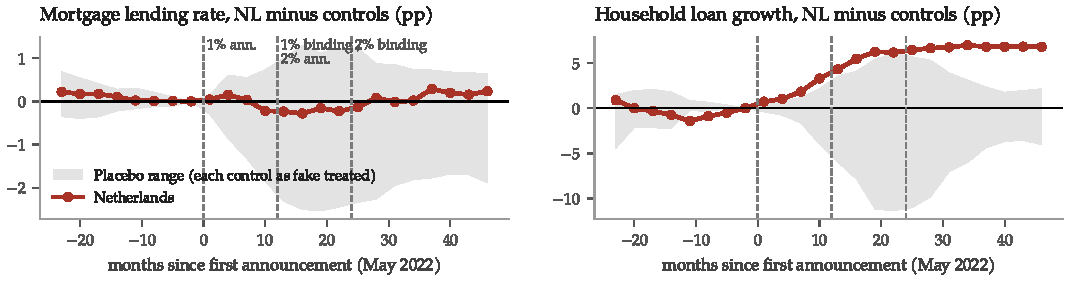
\includegraphics[width=\textwidth]{figs/event.pdf}\par
  \raggedright\small\vspace{2pt}
  We compare the Netherlands with five euro-area countries that never changed their buffer (Austria, Finland, Italy, Malta, Luxembourg). The red line is the Dutch difference; the grey band shows differences that arise by chance when each control country is treated as if it had raised its buffer. Mortgage rates stayed inside the band, and household credit grew faster than in the controls, partly as a catch-up.
  \takeaway{We find \hl{no sign of contraction}, although this is not a causal estimate. DNB reached the same view in September 2026.}
  \source{ECB Data Portal (MIR, BSI); ESRB CCyB table (control selection); DNB press release 17 Sep 2026; own two-way fixed-effects event study with placebo inference.}
\end{frame}

% ===================================================================================== 17
\qtag{Q3 · Implications}
\begin{frame}{Nor did the buffer double the ECB's squeeze. It let monetary policy focus on inflation}
  \begin{columns}[T,onlytextwidth]
    \column{0.58\textwidth}
    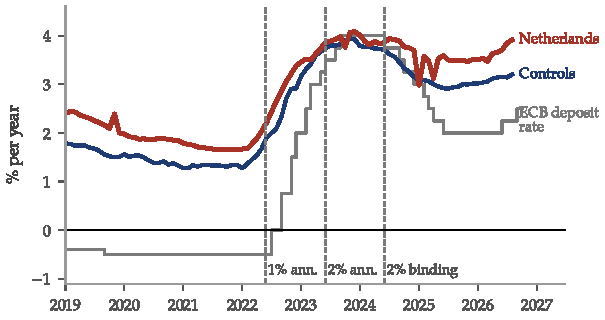
\includegraphics[width=\linewidth]{figs/rates.pdf}
    \column{0.38\textwidth}\small
    A natural worry is that two tightenings at once, higher policy rates and higher capital requirements, would choke credit. The chart shows that Dutch mortgage rates followed the ECB's rate and moved closely with those in the control countries.\\[5pt]
    The ECB argues that early CCyB activation {\itshape “helps monetary policy focus on its primary objective of price stability.”} {\footnotesize\color{grey}(ECB, 2025)}
  \end{columns}
  \takeaway{With one monetary policy for twenty countries, the CCyB is the Dutch-specific lever, and it is insurance in case a rate shock goes wrong.}
  \source{ECB Data Portal (MIR mortgage rates; deposit facility rate); ECB Macroprudential Bulletin 31 (Detken, Hempell \& Pirovano, 2025). Controls: AT, FI, IT, MT, LU.}
\end{frame}

% ===================================================================================== 18
\qtag{Q3 · Implications}
\begin{frame}{Through reciprocity the 2\% also binds foreign lenders, and the rest of Europe is moving the same way}
  \begin{columns}[T,onlytextwidth]
    \column{0.58\textwidth}
    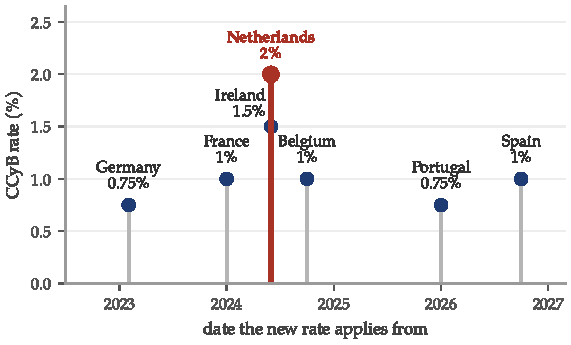
\includegraphics[width=\linewidth]{figs/europe.pdf}
    \column{0.38\textwidth}\small
    Under EU reciprocity, foreign banks that lend into the Netherlands must also hold the Dutch 2\% on those loans. This limits leakage to foreign lenders, a known weakness of national capital rules, although lending can still move to non-banks.\\[5pt]
    The Netherlands was early and set the highest rate, but it was not alone. Since 2023 Germany, France, Ireland, Belgium, Portugal and Spain have all raised their buffers.
  \end{columns}
  \takeaway{The Dutch move is part of a broader European shift towards keeping releasable capital in normal times.}
  \source{DNB press release 31 May 2023; ESRB CCyB rates table (Sep 2026); ECB Macroprudential Bulletin 21 (Behn et al., 2023); Aiyar, Calomiris \& Wieladek (2014).}
\end{frame}

% ===================================================================================== 19
\qtag{Q3 · Implications}
\begin{frame}{The result: next time, DNB can release €6.7bn overnight}
  \centering\vspace{4pt}
  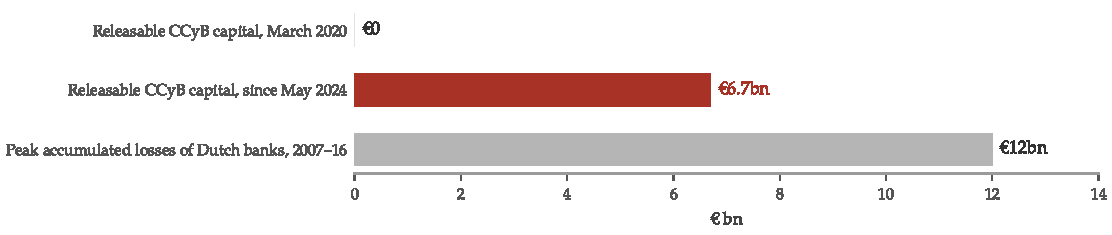
\includegraphics{figs/resilience.pdf}\par
  \raggedright\small\vspace{6pt}
  In March 2020 the Netherlands had no releasable capital. Today it has €6.7bn, about half of the peak losses after the financial crisis and enough to support up to €150bn of lending. Research suggests the payoff is asymmetric: a one-point increase in normal times reduces lending by only about 0.1\%, while a one-point release in bad times can raise it by up to 10\%.\\[3pt]
  With the mortgage risk-weight floor expiring in November 2026, DNB says this \emph{“underpins the importance of … the current countercyclical capital buffer (CCyB) of 2\%.”}
  \takeaway{The buffer is cheap to hold and powerful to release.}
  \source{DNB framework (2022); Lang \& Menno (2023), ECB WP 2828; DNB press release 24 Apr 2026.}
\end{frame}

% ===================================================================================== 20
\qtag{Q3 · Implications}
\begin{frame}{The price is reliance on discretion, and the buffer has never been tested}
  \small
  \renewcommand{\arraystretch}{1.35}
  \begin{tabularx}{\textwidth}{@{}L{3.2cm}X@{}}
    \toprule
    \textbf{Credibility} & Without a mechanical rule, markets must trust DNB's judgement, so DNB has to explain every decision. This is the classic trade-off between rules and discretion (Kydland \& Prescott, 1977). \\
    \textbf{Calibration} & Why 2\% and not 1.5\%? The ECB's loss-based estimates range from 1.1\% to 1.8\%, so the Dutch rate sits at the top of the banking union. \\
    \textbf{Untested} & The buffer has never been released. Will banks lend the freed capital, or hoard it, as many did with usable buffers in COVID? \\
    \textbf{Baseline} & Compared with 2021 rather than 2019, the refill \emph{was} an increase: €3.3bn before the O-SII offset. \\
    \textbf{The same profits, twice} & The ECB lists the Netherlands among the countries that adopted levies on banks' excess profits in 2022--23. These levies partly claim the earnings that fund the buffer. \\
    \bottomrule
  \end{tabularx}
  \takeaway{None of these overturns the verdict, but they define what DNB must get right next time.}
  \source{Kydland \& Prescott (1977); De Nora et al.\ (2025); ECB Macroprudential Bulletin 21 (2023) and 31 (2025); DNB (2022, 2023).}
\end{frame}

% ===================================================================================== 21
\qtag{Conclusion}
\begin{frame}{In short, the promise was kept: the buffer was refilled in a storm, at the moment it was cheapest}
  \begin{columns}[T,onlytextwidth]
    \column{0.31\textwidth}
    \heading{Q1 · Environment}
    \footnotesize A recovered economy was hit by war, inflation and rate hikes. Credit was cold, housing was hot and then cooled, and the banks were strong and profitable.
    \column{0.31\textwidth}
    \heading{Q2 · Criteria and risks}
    \footnotesize A 2\% normal level, calibrated on past losses, insures against shocks nobody can forecast. Housing went to other tools, and structural buffers were cut in return.
    \column{0.31\textwidth}
    \heading{Q3 · Implications}
    \footnotesize The refill was cheap and largely a swap, with no sign of contraction. It complements monetary policy, binds foreign lenders and leaves €6.7bn releasable, at the price of discretion.
  \end{columns}
  \vspace{22pt}
  \begin{center}
    {\color{black!25}\rule{0.55\textwidth}{0.3pt}}\\[12pt]
    {\Large\color{navy} In March 2020, the Netherlands had nothing to release.\\[4pt] Next time, it will.}\\[12pt]
    {\itshape The best time to fill a buffer is when nobody thinks you need it, even in a storm.}\\[10pt]
    {\color{black!25}\rule{0.55\textwidth}{0.3pt}}
  \end{center}
\end{frame}

% ===================================================================================== Glossary (backup)
\qtag{Appendix}
\begin{frame}{Glossary}
  \fontsize{7.6}{9.2}\selectfont
  \begin{columns}[T,onlytextwidth]
    \column{0.49\textwidth}
    \begin{tabularx}{\linewidth}{@{}>{\raggedright\arraybackslash\bfseries}p{2.3cm}X@{}}
      \toprule
      CCyB & Countercyclical capital buffer: 0–2.5\% of risk-weighted assets on domestic exposures; raised with a 12-month lag, released immediately. \\
      Positive neutral CCyB & A CCyB kept above zero when risks are neither high nor low, so it can be released for any shock. \\
      CET1 & Common Equity Tier 1: the highest-quality capital (shares, retained earnings), as \% of RWA. \\
      RWA & Risk-weighted assets: assets weighted by their riskiness (e.g.\ mortgages count less than corporate loans). \\
      Pillar 1 / P2R / P2G & Legal minimum (4.5\% CET1) / bank-specific add-on set by the supervisor / non-binding supervisory guidance. \\
      CCoB & Capital conservation buffer, 2.5\% for all banks. \\
      O-SII / SRB & Buffer for other systemically important institutions / systemic risk buffer (structural, not designed for release). \\
      MDA & Maximum distributable amount: if CET1 falls below the combined buffer requirement, payouts are automatically restricted. \\
      \bottomrule
    \end{tabularx}
    \column{0.49\textwidth}
    \begin{tabularx}{\linewidth}{@{}>{\raggedright\arraybackslash\bfseries}p{2.3cm}X@{}}
      \toprule
      Credit-to-GDP gap & Credit/GDP ratio minus its long-run trend; the Basel reference for the CCyB (gap 2–10pp → buffer 0–2.5\%). \\
      HP filter & Hodrick-Prescott filter: estimates a smooth trend; one-sided uses only past data (real time), two-sided also future data. \\
      Headroom & CET1 capital above a bank's requirement / MDA trigger. \\
      Reciprocity & Foreign banks must apply the Dutch CCyB rate to their Dutch exposures. \\
      Borrower-based measures & Limits on loan-to-value (LTV) and loan-to-income (LTI) of new mortgages. \\
      Risk-weight floor & Minimum average risk weight on Dutch mortgages of banks using internal models (Art.\ 458 CRR), Jan 2022 – Nov 2026. \\
      Event study / placebo & Compare NL with countries that did not change their CCyB around each date / repeat with each control as a fake “treated” country. \\
      pp / bp & Percentage point / basis point (0.01pp). \\
      \bottomrule
    \end{tabularx}
  \end{columns}
\end{frame}

% ===================================================================================== 22
\qtag{Appendix}
\begin{frame}{Methods and references}
  \fontsize{6.6}{7.7}\selectfont
  \textbf{Methods.} Credit gap: one-sided (recursive) and two-sided HP filter, $\lambda=400{,}000$, sample from 1961Q1; Hamilton (2018) regression filter, $h=8,20$, $p=4$. Headroom: (CET1 ratio − CET1 requirement/MDA) × total RWA per bank; CCyB amount sector-wide (upper bound); 6–47\% assumption grid as sensitivity. Event study: two-way FE, NL × 3-month event-time bins, country and month FE; placebo inference over controls with no CCyB change 2021–25. Code and data: GitHub repository (code/, data/).\par\medskip
  \begin{columns}[T,onlytextwidth]
    \column{0.49\textwidth}
    \textbf{Primary sources}\par
    BCBS (2024). Range of practices in implementing a positive neutral CCyB (d585).\par
    DNB (2020). DNB lowers bank buffer requirements to support lending, 17 Mar.\par
    DNB (2022). Analytical framework for setting the CCyB in the Netherlands.\par
    DNB (2022, 2023). CCyB press releases, 27 May 2022, 31 May 2023; O-SII news item, 31 May 2023.\par
    DNB (2026). CCyB decisions 26 Mar and 17 Sep; risk-weight measure expires, 24 Apr.\par
    DNB. Financial Stability Report, spring 2022 and spring 2023.\par
    Knot, K. (2023). Introductory statement, Standing Parliamentary Committee for Finance, 7 Jun.\par
    ECB (2020). Temporary capital and operational relief, 12 Mar; ECB (2022). Monetary policy decisions, 21 Jul.\par
    ESRB. CCyB rates table; O-SII notifications NL (27 Nov 2020; 31 May 2023); COVID-19 measures.\par
    Data: BIS (credit gaps, total credit, DSR, property prices); ECB Data Portal (MIR, BSI); CBS; bank annual and Pillar 3 reports (ING, Rabobank, ABN AMRO, de Volksbank).\par
    \column{0.49\textwidth}
    \textbf{Literature}\par
    Aiyar, Calomiris \& Wieladek (2014). Does macro-prudential regulation leak? \emph{JMCB} 46(s1).\par
    Behn, Pereira, Pirovano \& Testa (2023). A positive neutral rate for the CCyB. \emph{ECB MPB} 21.\par
    Couaillier, Lo Duca, Reghezza \& Rodriguez d'Acri (2022). Caution: do not cross! \emph{ECB WP} 2644.\par
    De Nora, Pereira, Pirovano \& Stammwitz (2025). From losses to buffer. \emph{ECB WP} 3061.\par
    Detken, Hempell \& Pirovano (2025). Macroprudential and monetary policy interaction. \emph{ECB MPB} 31.\par
    Drehmann, Borio, Gambacorta, Jiménez \& Trucharte (2010). Countercyclical capital buffers: exploring options. \emph{BIS WP} 317.\par
    Edge \& Meisenzahl (2011). The unreliability of credit-to-GDP ratio gaps in real time. \emph{IJCB} 7(4).\par
    Hamilton (2018). Why you should never use the Hodrick-Prescott filter. \emph{REStat} 100(5).\par
    Herrera, Scalone \& Pirovano (2024). The importance of being positive. \emph{ECB MPB} 24.\par
    Kydland \& Prescott (1977). Rules rather than discretion. \emph{JPE} 85(3).\par
    Lang \& Menno (2023). The state-dependent impact of changes in bank capital requirements. \emph{ECB WP} 2828.\par
    Repullo \& Saurina (2011). The countercyclical capital buffer of Basel III: a critical assessment. CEMFI WP 1102.\par
    Tinbergen (1952). \emph{On the Theory of Economic Policy}. North-Holland.\par
  \end{columns}
\end{frame}

\end{document}
